\chapter{Fundamentação teórica}
\label{cap:fundamentos}

% figuras estão no subdiretório "figuras/" dentro deste capítulo
\graphicspath{\currfiledir/figuras/}

%=====================================================

%\section{}

Este capítulo revisita os tópicos fundamentais deste trabalho, incluindo os princípios de redes neurais adversariais, evolução de variável latente e algoritmos genéticos para exploração do espaço latente com o exemplo do CMA-ES; explora a literatura no tópico de geração de conteúdo procedural utilizando aprendizado de máquina; e apresenta o principal artigo que guiou este trabalho, que utiliza uma DCGAN para gerar níveis do jogo Super Mario Bros.(1985). 

%=====================================================

\section{Redes Neurais Adversariais Generativas}

O paradigma do Aprendizado Adversarial e as Redes Neurais Adversariais Generativas (GANs) foram introduzidos em \cite{gan} em 2014 como solução para o problema de estimação de máxima verossimilhança, dilema no qual o custo computacional e a complexidade são extremamente altos, podendo chegar a ser computacionalmente inviável a depender do contexto. Enquanto a gama mais popular de modelos profundos na época de publicação do artigo consistiam de apenas uma rede neural de alta profundidade usada em classificação e, em certos casos, regressão, o aprendizado adversarial proposto pelo artigo usufrui de duas MLPs.

Um desses modelos é apelidado de gerador, abreviado como \textit{G}, enquanto o outro modelo é chamado de discriminador e abreviado como \textit{D}. O modelo gerador representa uma função diferenciável responsável por aproximar a distribuição de seus dados de treinamento. Para gerar novos dados, a rede \textit{G} projeta entradas ruidosas no espaço dos dados conhecidos, na intenção de aproximar o conteúdo gerado da distribuição dos conjuntos conhecidos.

Por sua vez, a MLP \textit{D} tem como objetivo traçar um plano que separe as distribuições do conteúdo original das distribuições das projeções de \textit{G}. A saída da rede discriminadora, no artigo, é descrita como um único escalar que representa a probabilidade de uma entrada não ser gerada. Essencialmente, \textit{G} e \textit{D} tornam-se antagônicas a partir do momento que suas respectivas funções de perda colocam como objetivo penalizar a outra. Para que isso seja possível, \textit{G} é treinada para minimizar $\log_ (1-D(G(z)))$ enquanto \textit{D} é treinada para maximizar a probabilidade de acertar se uma entrada é sintética ou real. Este treinamento antagônico leva essas duas redes a disputarem um jogo MinMax de dois jogadores. Alternando a otimização de \textit{D} e \textit{G}, a rede discriminadora fica mais perto da solução ótima, enquanto a MLP geradora muda aos poucos para sua distribuição aproximar cada vez mais da original e, por consequência, tornar a solução que o discriminador busca mais complexa de se aproximar. 

%=====================================================

\section{CMA-ES}

CMA-ES, a \emph{Covariance Matrix Adaptation Evolution Strategy}, foi instanciada primeiro em \cite{cma-es}. É uma estratégia evolucionária que se comporta bem com vetores de números reais, que neste casos são as entradas do gerador, e sua principal característica é o uso de uma matriz de covariância estimada iterativamente por diferenças finitas.

Como está no seu nome, o algoritmo faz parte de um grupo de algoritmos evolucionários chamados \emph{evolutionary strategies}, que é um grupo de algoritmos caixa preta caracterizados também pelo uso da ordenação por ranking. A CMA-ES tem se mostrado eficiente para otimizar problemas não-convexos e não-lineares em domínios contínuos.

O que este algoritmo faz é calcular uma gaussiana com base na matriz de covariância estimada. Esta gaussiana é traduzida numa elipse que se desloca de forma a contemplar as melhores soluções. Quanto mais distantes as melhores soluções estão do domínio dessa elipse, maior o \emph{step size} dela, ou seja, seu raio. De certa forma, no começo, o \emph{step size} costuma ser mais alto pois as melhores soluções conhecidas estão esparsas e a partir deste ponto de partida há a exploração global. Conforme a elipse fica melhor posicionada no domínio, as melhores soluções ficarão menos esparsas, fazendo com que o \emph{step size} diminua proporcionalmente com a concentração da população.

Segue um pseudo-código do que seria o CMA-ES:

\begin{algorithm}
\caption{CMA-ES}
\begin{algorithmic}[1]

\State Inicialize a população: $\lambda$
\State Inicialize o \texit{step size}: $\sigma$
\State Defina o tamanho da população: $m$

\State defina o número de melhores candidados $\mu$

\State Defina os pesos: $W_1, W_2, \ldots, W_m$

\State \textbf{repeat}
\ForAll{$x \in \lambda$}
  \State Calcula a gaussiana para $x$
\EndFor

\State Ordena $\lambda$ pelo fitness

\State $c \gets calcula_covariancia(\lambda)$

\State $m \gets \sum_{i=1}^{\mu} W_i \cdot X_i$

\State $\sigma \gets$ atualiza($\sigma$)

\State \textbf{until} número de iterações $>$ $max\_iter$

\end{algorithmic}
\end{algorithm}

%A atualização do \emph{step size} pode ser encontrada nas páginas 20, 29 e 31 do tutorial feito pelo autor original do CMA-ES \cite{manual_cma-es}.

%=====================================================

\section{Evolução de Variavel Latente (LVE)}

LVE - \emph{Latent Variable Evolution} - surgiu primeiro para buscar digitais específicas num certo espaço mapeado por uma GAN em \cite{fingerprints}. Como dito anteriormente, a rede neural geradora de uma GAN mapeia entradas ruidosas para um espaço. Estas entradas ruidosas também são chamadas de variáveis latentes, ou seja, variáveis que são difíceis ou impossível de controlar e interpretar antes de um resultado concreto.

A partir disso, a técnica de LVE tem como ideia manipular as entradas ruidosas de um modelo para que sua saída se encaixe dentro de certas especificações, ou seja, adiciona ao conteúdo gerado restrições que até o momento atual não são controláveis a nível de treinamento, pois uma rede geradora tem como única função reproduzir a distribuição de seus dados de teste. Em \cite{fingerprints}, a técnica de LVE é utilizada para a quebra de identificação de digitais. A técnica consiste de duas etapas: primeiro, treinar uma rede neural para gerar o conteúdo alvo e, após isso, usar um algoritmo para buscar no espaço latente uma entrada que gere uma saída dentro das condições especificadas.

O algoritmo utilizado por \cite{fingerprints} para busca no espaço latente é o já explicado anteriormente CMA-ES. A justificativa do uso do CMA-ES pelo autores é que a função objetivo é não contínua e, pela natureza de redes convolucionais, também não é linearmente separável.

%\cite{marioGAN} diz que GANs são "compactos e robustos mapeamentos genótipos-fenótipos". Nesta interpretação, em que genótipos são as entradas e os fenótipos as saidas correspondentes, é possível manipular os fenótipos para que os genótipos se encaixem dentro de algo desejado, ou seja, manipular as entradas para que a GAN produza a saída desejada. Para isso, o método explorado pelo paper da MarioGAN é o CMA-ES.

%Ao elaborar o texto da dissertação ou da tese, o mais indicado é o uso do verbo na forma impessoal. Exemplos:

%\begin{itemize}
%\item ... utilizaram-se os seguintes dados ...
%\item ... elaborou-se de forma precisa ...
%\item ... trata-se os algoritmos ...
%\item ... foram obtidos resultados significativos ...
%\end{itemize}

%Além disso, deve-se a todo custo evitar a ``linguagem de revista'', com expressões como ``sensacional'', ``impressionante'', ``monstruoso'', etc (por exemplo: ``Os resultados obtidos são sensacionais, sobretudo considerando a monstruosa margem de erro.'').

%=====================================================

\section{Geração de Conteúdo Procedural Usando Aprendizado de Máquina (PCGML) }

A survey de Summerville e colegas \cite{survey2018} define \emph{Procedural Content Generation Via Machine Learning} como "geração de conteudo de jogos usando modelos de \emph{machine learning} em conteúdos existentes". Na área, busca-se aumentar o valor de replay, salvar memória, reduzir o custo e o esforço de produção, diversificar estética e reduzir a presença humana na geração de conteúdo de jogos. Na área acadêmica, além disso, pode-se dizer que se explora novas maneiras de experenciar os jogos, além de ser um desafio que estimula a criatividade computacional e o entendimento de \emph{game design} pela construção de modelos.

%=====================================================

\section{NSGA-II}

Em Abril de 2002 foi proposto a evolução do \textit{nondominated sorting genetic algorithm} (algoritmo genético de ordenção não-dominada), o NSGA-II\cite{Deb:02}, que hoje em dia conta com 37971 citações(Connected Papers, acesso em 05/11/2023). Esse algoritmo foi proposto na intenção de contornar os três principais problemas dos algoritmos evolucionários apontados na época:

\begin{itemize}
    \item Alta complexidade computacional(especificamente $O(MN^{3})$, onde M é o numero de objetivos e N o tamanho da população);
    \item A falta de elitismo;
    \item A necessidade de especificar parâmetros, como o caso do NSGA proposto em \cite{Deb:94};
\end{itemize}

E sua implementação nos permite:

\begin{itemize}
    \item Preservar a diversidade;
    \item e enfatizar soluções não-dominadas.
\end{itemize}

Tendo populaçoes de tamanho N, o NSGA-II recombina tal população numa população de tamanho 2N e a ordena baseado no ranking da fronteira de pareto, priorizando soluções da fronteira classe 1 e completando com as fronteiras subsequentes. Quando a fronteira $F_{g}$ nao cabe mais inteira na próxima população, são selecionadas os indivíduos com maior \texit{crowd distance}, que é a área/volume (dependente do tamanho do espaço objetivo $Z$ do problema) ao seu redor sem nenhuma solução presente (cabe enfatizar que as funções objetivo são normalizadas para que nenhuma domine a outra). Este operador permite escolher as soluções que estão mais distantes das outras, por consequência também sendo um preservador de diversidade por si só.

%=====================================================

\section{PSO}

Otimização por enxames de partículas foi proposta por \cite{PSO}. Segundo os autores, é um método de otimização para funções contínuas e não-lineares que simula um modelo social simplificado. O algoritmo instância uma população candidata e a move pelo domínio de acordo com fórmulas matemáticas simples em relação a posição e velocidade da partícula. 

A metaheurística associada ao PSO faz pouca ou nenhuma suposição do problema que será otimizado. Outra vantagem é que o algoritmo não utiliza otimização por gradiente como muitos dos algoritmos de computação evolutiva, o que significa que a função objetivo não precisa ser diferenciável. 
%=====================================================

\section{Algoritmo A estrela}

O algoritmo A estrela é uma extensão do Algoritmo de Djikstra que utiliza alguma metaheurística para guiar a busca pelo caminho mais curto ao objetivo. Para que o algoritmo funcione corretamente, a heurística definida para auxiliar a busca deve ser admissível, isto é, o custo estimado para atingir o estado final em relação ao estado atual deve ser menor ou igual ao custo verdadeiro para atingir o estado final do estado atual. 

A busca A estrela possui múltiplas aplicações, entre elas a busca por caminhos viáveis em videogames. Até os dias de hoje, o mais popular algoritmo para o teste de jogabilidade de níveis do jogo \textit{Super Mario Bros} é o agente A* proposto por Robin Baumgarten em \cite{marioAI}.

%=====================================================

\section{MarioGAN}

Em maio de 2018 publicou-se o artigo que deu origem ao que outros entusiastas do estudo da PCGML chamam de MarioGAN \cite{marioGAN}. O artigo aborda o uso de GANs, mas não foca na arquitetura da rede geradora ou discriminadora, mas sim utiliza a ideia de LVE para geração de níveis procedurais no jogo \emph{Super Mario Bros}. Aqui, seguindo a ideia de \cite{fingerprints}, o CMA-ES é utilizado para adicionar alguma restrição ao espaço latente do gerador, sendo testadas quatro funções-objetivo diferentes, duas delas relacionadas a disposição dos blocos da fase e outras duas em relação ao teste das fases pelo agente A* vencedor da competição Mario AI de 2009\cite{marioai} de autoria de Robin Baumgarten.

Para representar as fases, os autores utilizaram a representação do jogo \textit{Super Mario Bros} disponível no repositório do \textit{github} aberto da Video Game Level Corpus(VGLC) \cite{VGLC}, que, entre suas particularidades, simplificam a representação do jogo ao ignorar níveis específicos, onde a física do jogo diverge do padrão seguido pela maioria das fases, e também representa todos os inimigos da mesa maneira, tornando a tarefa possivelmente mais simples. Nesta representação, cada tipo de bloco é mapeado para um caracter específico, transformando a imagem em uma sequência de caracteres que indicam um bloco específico. Uma vez que o artigo implementa a arquitetura a partir da biblioteca \textit{Pytorch}, esta representação textual precisou ser remapeada para uma representação numérica, conforme mostrado pela \textbf{Figura 2.1}. 

\begin{figure}[!htb]
\centering
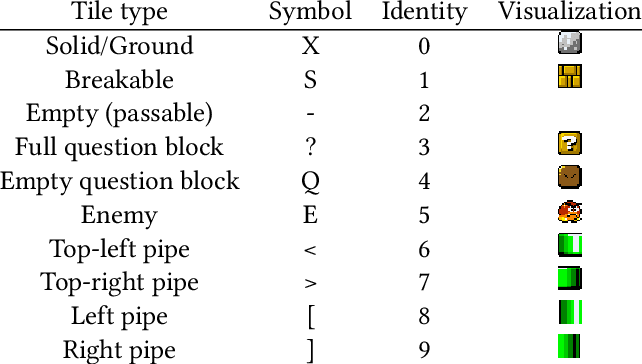
\includegraphics[width=12cm]{imagens/representacao_mario.png}
\caption{Representação dos elementos do jogo \textit{Super Mario Bros} pela VGLC e pelos autores de \cite{marioGAN}, respectivamente. Fonte: \cite{marioGAN} }
\label{fig:2.1}
\end{figure}

A GAN convolucional profunda (DCGAN) utilizada no artigo é baseada na Wassertein Gan apresentada em \cite{wgan}, em que o discriminador utiliza convoluções com deslocamento (\textit{strided convolutions} ), enquanto o gerador utiliza convoluções com deslocamento fracionário (\textit{fractional-strided convolutions}. A arquitetura em \cite{marioGAN} difere de \cite{WGAN} nos seguintes pontos:

\begin{itemize}

	\item Tanto no discriminador quanto no gerador, é empregada uma camada de normalização de bloco (\textit{batch normalization} após cada camada convolucional;

	\item A função de ativação de todas as camadas (inclusive na de saída) é a ReLU (O discriminador, como em \cite{wgan}, utiliza a Leaky ReLU como função de ativação em suas camadas).

\end{itemize}

Tanto o discriminador quanto o gerador são treinados com o otimizador RMSprop, com um \textit{batch size} de tamanho 32 e a taxa de aprendizado de 0,00005 por 5000 iterações. A arquitetura é devidamente ilustrada na \textbf{Figura 2.2}.

\begin{figure}[!htb]
\centering
	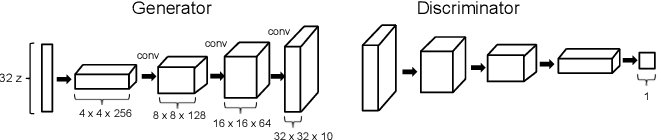
\includegraphics[width=12cm]{imagens/arquitetura_mariogan.png}
	\caption{Representação da arquitetura da GAN utilizada no paper. Fonte: \cite{marioGAN}}
\label{fig:2.2}
\end{figure}

O gerador utilizado no artigo é treinado apenas com o primeiro nível do jogo, na intenção de mostrar como a LVE e a GAN treinada poderiam, em conjunto, gerar níveis diferentes e jogáveis. Outra escolha interessante do artigo da MarioGAN \cite{marioGAN} é que, para gerar múltiplas amostras com apenas uma fase, a representação numérica foi separada com base em uma janela deslizante com dimensões de 14 de altura e 28 de largura, com passo de tamanho um. 

Uma noção geral do processo executado por \cite{marioGAN} está devidamente traduzido na \textbf{Figura 2.3}. Este método é dividido em duas fases básicas distintas: primeiro, a WGAN é treinada de maneira não-supervisionada para gerar níveis do \textit{Super Mario Bros}; após isso, o CMA-ES é utilizado de forma a buscar no espaço latente da GAN, ou seja, alterar a entrada do modelo para satisfazer propriedades específicas. Embora o artigo se baseie apenas em níveis do jogo \textit{Super Mario Bros}, os autores clamam que o modelo é suficientemente bom para generalizar qualquer jogo com representação compatível.

\begin{figure}[!htb]
\centering
        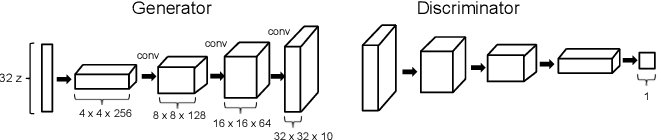
\includegraphics[width=12cm]{imagens/arquitetura_mariogan.png}
	\caption{Representação do processo de treinamento e de LVE. Fonte: \cite{marioGAN}}
\label{fig:2.3}
\end{figure}

Quanto as funções minimizadas em relação a topologia do nível minimizadas no artigo, as equações (1) e (2) as traduzem, em que g e t são respectivamente a fração da quantidade de blocos de chão na ultima linha da matriz que representa a fase e a fração desejada, e n o número de inimigos.

\begin{equation}
    F_1 = \sqrt{(g - t)^2}
\end{equation}

\begin{equation}
    F_2 = F_1 + 0.5 \cdot (20.0 - n)
\end{equation}

No artigo, a ideia apresentada é que a dificuldade aumente gradativamente conforme a progressão no eixo x, lembrando que o objetivo do jogo é chegar ao fim da fase, ou seja, no último ponto do eixo x. Para isso, os autores juntam dois níveis otimizados com $F_1$ e $t = 1$, um nível otimizado com $F_1$ e $g = 0.7$, e dois níveis otimizando $F_2$ com $g = 0.7$. O exemplo desta junção está na \textbf{Figura 2.3}.

\begin{figure}[!htb]
\centering
	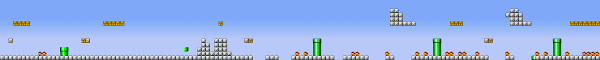
\includegraphics[width=12cm]{imagens/nivel_gerado.png}
        \caption{Nível gerado pelos autores, com progressão de dificuldade no eixo x. Fonte: \cite{marioGAN}}
\label{fig:2.3}
\end{figure}

Em outros experimentos, os autores usam duas funções relacionadas ao teste pelo agente A estrela vencedor da competição da marioAI de 2009, conforme as equações (3) e (4), onde p é a fração da fase em que o agente passou, e #jumps a quantia de pulos:

\begin{equation}
    F_3 =
    \begin{cases}
        -p, & \text{se } p < 1, \\
        -p - \#jumps, & \text{se } p = 1.
    \end{cases}
\end{equation}

\begin{equation}
    F_4 =
    \begin{cases}
        -p + 60, & \text{se } p < 1, \\
        -p + \#jumps, & \text{se } p = 1.
    \end{cases}
\end{equation}

Na verdade, $F_3$ maximiza os pulos e recompensa fases passáveis, enquanto $F_4$ também recompensa fases jogáveis, mas minimizando pulos. A \textbf{Figura 2.4} ilustra alguns desses níveis gerados.

\begin{figure}[!htb]
\centering
        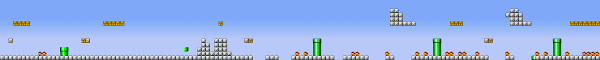
\includegraphics[width=12cm]{imagens/nivel_gerado}
        \caption{Nível gerado pelos autores, de acordo com a performance do agente. A letra a utiliza $F_3$, enquanto a parte b utiliza $F_4$. Fonte: \cite{marioGAN}}
\label{fig:2.4}
\end{figure}

Lembrando que não foram feitas abordagem multi-objetivo utilizando $F_1$ ou $F_2$ e $F_3$ ou $F_4$.

%=====================================================

\section{Conclusão}

Neste capítulo, foram apresentados os conceitos de GAN, PCGML e LVE, além de três algoritmos bioinspirados - CMA-ES, PSO e NSGA-II - que se relacionarão diretamente aos demais conceitos no decorrer do trabalho. Também foi apresentado o algoritmo A estrela, que será utilizado para teste e otimização das fases, além de uma visão ampla de um dos principais artigos da área de PCGML, artigo em que a rede proposta ficou conhecida como \textit{MarioGAN}. No próximo capítulo, serão visitados alguns outros artigos da área, muitos os quais utilizam de alguma forma os conceitos aqui apresentados.


%\subsection{Exemplo de figura}

%A forma sugerida para incluir figuras em um documento \LaTeX\ é importá-las usando o pacote \texttt{graphicx}. Como formatos gráficos sugere-se:

%\begin{itemize}

%\item Formatos \emph{raster}, como PNG (\emph{Portable Network Graphics}) ou JPG (\emph{Joint Photographic Experts Group}) para fotografias; procure usar uma resolução de ao menos 150 dpi (\emph{dots per inch}).

%\item Formatos vetoriais, como PDF (\emph{Portable Document Format}) ou EPS (\emph{Extended PostScript}) para diagramas e gráficos\footnote{NUNCA use JPG ou GIF para desenhos vetoriais, pois o resultado final geralmente fica borrado.}.

%\end{itemize}

%A maior parte das ferramentas permite exportar figuras nesses formatos (a figura do exemplo foi produzida com o \emph{Inkscape}, um programa livre multiplataforma). A figura \ref{fig:comun-intra-inter} mostra um exemplo de inclusão de figura em PDF.

% exemplo de inserção de figura
%\begin{figure}[!htb]
%\centering
%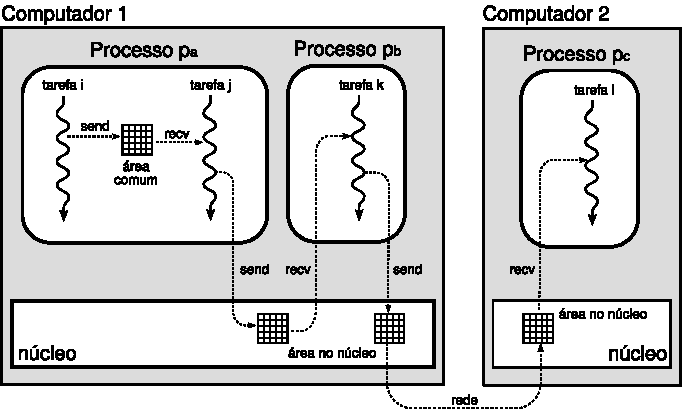
\includegraphics[width=12cm]{exemplo-figura.pdf}
%\caption{Comunicação inter-processos.}
%\label{fig:comun-intra-inter}
%\end{figure}

%Para mais informações consulte \cite{goossens93}.

%=====================================================

%\subsection{Exemplo de tabela}

%Tabelas são elementos importantes de um documento. No \LaTeX\ as tabelas podem ser objetos flutuantes (definidas no ambiente \texttt{table} e referenciadas por números usando \texttt{label} e \texttt{ref}) ou objetos fixos simples, criados pelo ambiente \texttt{tabular}. A tabela \ref{tab:modelos} é um exemplo de tabela flutuante, cuja posição no texto pode variar em função das quebras de página.

%\begin{table}[!htp]
%\centering
%\caption{Os 16 modelos centrais do UCON$_{\mathrm{ABC}}$}
%\label{tab:modelos}
%\begin{tabular}{|c|cccc|}
%\cline{2-5}
%\multicolumn{1}{c|}{}& 0 (imutável) & 1 (\emph{pre-update}) & 2 (\emph{on-update}) & 3 (\emph{pos-update}) \\
%\hline
%\texttt{preA} & \textbullet & \textbullet & -- & \textbullet \\
%\hline
%\texttt{onA} & \textbullet & \textbullet & \textbullet & \textbullet \\
%\hline
%\texttt{preB} & \textbullet & \textbullet & -- & \textbullet \\
%\hline
%\texttt{onB} & \textbullet & \textbullet & \textbullet & \textbullet \\
%\hline
%\texttt{preC} & \textbullet & -- & -- & -- \\
%\hline
%\texttt{onC} & \textbullet & -- & -- & -- \\
%\hline
%\end{tabular}
%\end{table}

%=====================================================

%\subsection{Exemplo de fórmula}

%Equações destacadas devem ser numeradas como mostra a equação \ref{eq:relatividade}:

%\begin{equation}
%E = m \times c^2
%\label{eq:relatividade}
%\end{equation}

%=====================================================

%\subsection{Exemplos de código-fonte}

%Códigos-fonte podem ser produzidos de forma simples através do ambiente \texttt{verbatim}, como mostra este exemplo:

%\begin{footnotesize}
%\begin{verbatim}
%#include <stdio.h>

%int main (int argc, char *argv[])
%{
%   int i ;                           // uma variavel local
%
%   for (i=0; i< 100; i++)            // um laço for
%      printf ("i vale %d\n", i) ;    // uma saída na tela
%}
%\end{verbatim}
%\end{footnotesize}

%No entanto, é preferível usar pacotes especializados para a edição ou inclusão de códigos-fonte, como o pacote \texttt{listings}. Eis um exemplo de código-fonte escrito com esse pacote:

% exemplo de código-fonte definido no próprio texto

%\begin{lstlisting}
%#include <stdio.h>

%int main (int argc, char *argv[])
%{
  % int i ;                           // uma variável local

 %  for (i=0; i< 100; i++)            // um laço for
%      printf ("i vale %d\n", i) ;    // uma saída na tela
%}
%\end{lstlisting}

%Esse pacote também permite incluir códigos-fonte de arquivos externos. Eis um exemplo:

% exemplo de código-fonte incluso

%\lstinputlisting{2-fundam/exemplo.c}

%=====================================================

%\subsection{Exemplo de algoritmo}

%Os pacotes \texttt{algorithm} e \texttt{algorithmic} permitem formatar algoritmos facilmente. Eis um exemplo:

%\begin{algorithm}[H]
%\caption{Ações de $s_i$ ao encerrar um ciclo:}
%\label{alg:on-period-ending}
%\begin{small}
%\begin{algorithmic}[1]
%\FORALL{$x \in \mathcal{K}_i$}
%  \STATE{$\mathit{banned}_i(x) \gets$ FALSE}
%  \STATE{$mi_i(x) \gets 0$}
%  \STATE{$mm_i(x) \gets 0$}
%  \STATE{$\mathit{age}_i(x) \gets \mathit{age}_i(x) + 1$}
%  \IF{$\mathit{age}_i(x) = \mathit{age}_\mathit{max}$}
%     \STATE{$\mathcal{K}_i \gets \mathcal{K}_i - \{x\}$}
%     \COMMENT{``esquece'' do servidor $x$}
%     \STATE{remove as informações locais sobre $x$}
%     \STATE{envia $\mathit{notify}(x,\mathit{undef})$ ao grupo de confiança $\mathcal{T}_i$}
%  \ENDIF
%\ENDFOR
%\end{algorithmic}
%\end{small}
%\end{algorithm}
 
%=====================================================

%\subsection{Exemplos de citação}

%Citação curta (só um parágrafo): como afirmou Maquiavel em seu livro \emph{O Príncipe}:

%\begin{quote}
%``Nada é mais difícil de instituir, mais perigoso de conduzir, mais incerto no seu sucesso, do que liderar a introdução de uma nova ordem de coisas... O inovador faz inimigos em todos aqueles que prosperavam sobre as antigas regras, e somente tíbio suporte é esperado daqueles que prosperariam na novidade, porque os homens são geralmente incrédulos, nunca realmente confiam nas coisas novas, a menos que as tenham testado em experiência''.
%\end{quote}

%Citação longa (mais de um parágrafo): como afirmou Maquiavel em seu livro \emph{O Príncipe}:

%\begin{quotation}
%``Nada é mais difícil de instituir, mais perigoso de conduzir, mais incerto no seu sucesso, do que liderar a introdução de uma nova ordem de coisas...

%O inovador faz inimigos em todos aqueles que prosperavam sobre as antigas regras, e somente tíbio suporte é esperado daqueles que prosperariam na novidade, porque os homens são geralmente incrédulos, nunca realmente confiam nas coisas novas, a menos que as tenham testado em experiência''.
%\end{quotation}

%=====================================================

%\section{Uma seção}

%\subsection{Uma subseção}

%\subsubsection{Uma subsubseção}

%=====================================================

%\section{Conclusão}
%
%Todo capítulo (com exceção da introdução e da conclusão) deve encerrar com uma pequena conclusão local, resumindo os tópicos apresentados no capítulo e preparando o leitor para o próximo capítulo (exceto se esse for a conclusão geral). Caso o capítulo tenha apresentado resultados obtidos pelo próprio autor, estes devem ser sucintamente relembrados aqui.

%=====================================================
